% !TeX program = xelatex
% 编译：xelatex 04-离散LTI系统卷积公式推导.tex（VS Code 的 LaTeX Workshop 会读上一行，自动用 xelatex）
% 来源：2022 浙江大学《信号与系统》胡浩基老师，第二章「LTI 系统时域分析」，教材第 45 页 2.2 节，视频 00:00--107:46（整段视频）。
% 体例：从画图题出发逐步加难度，推广出卷积公式，再讲两种算法。
\documentclass[UTF8,a4paper,11pt]{ctexart}
\usepackage{amsmath,amssymb}
\usepackage{geometry}
\geometry{margin=2.4cm}
\usepackage{xcolor}
\usepackage{mdframed}
\usepackage{booktabs}
\usepackage{needspace}
\usepackage{array}
\usepackage{longtable}
\usepackage{enumitem}
\usepackage{tikz}
\usetikzlibrary{arrows.meta,positioning,calc}
\usepackage{float}
\usepackage{fancyhdr}
% 页眉页脚清空，只在右下角保留页号（含首页）
\fancypagestyle{plain}{%
  \fancyhf{}%
  \fancyfoot[R]{\thepage}%
  \renewcommand{\headrulewidth}{0pt}%
  \renewcommand{\footrulewidth}{0pt}}
\usepackage[hidelinks,unicode,bookmarksnumbered,bookmarksopen=true,bookmarksopenlevel=2,pdftitle={离散 LTI 系统卷积公式推导}]{hyperref}
\usepackage{bookmark}% XeTeX 下 hyperref 自带的大纲不生效，用 bookmark 宏包生成 PDF 书签（需编译两遍）

\setCJKmainfont{Songti SC}[BoldFont={Songti SC Bold}]
\setCJKsansfont{PingFang SC}

\newmdenv[backgroundcolor=blue!4,linecolor=blue!50!black,linewidth=1pt,innertopmargin=6pt,innerbottommargin=6pt]{rememberbox}
\newenvironment{remember}{\begin{rememberbox}\textbf{重点}\par\smallskip}{\end{rememberbox}}
\newmdenv[backgroundcolor=yellow!8,linecolor=orange!70!black,linewidth=1pt,innertopmargin=6pt,innerbottommargin=6pt]{notebox}
\newenvironment{note}{\begin{notebox}\textbf{说明}\par\smallskip}{\end{notebox}}
\newmdenv[backgroundcolor=gray!8,linecolor=gray!60,linewidth=0.8pt,innertopmargin=5pt,innerbottommargin=5pt]{skipbox}
\newenvironment{skippable}{\begin{skipbox}\textbf{可跳过}\par\smallskip}{\end{skipbox}}

% ---------------------------------------------------------------- 画图用的小宏
% 火柴杆图(stem plot)：在当前 tikzpicture 里、平移 (#1,#2) 处画一个离散序列。
% #3 起始下标，#4 从起始下标开始的取值列表（整数，逗号分隔），#5 纵向缩放(cm/单位)，
% #6、#7 横轴显示的下标范围。纵轴向上画 1.9cm，向下至少画 0.45cm（有更深的负值时画到它下面）。
% 横轴每个整数下标都有刻度；该点火柴杆朝下时，刻度数字挪到横轴上方，不压在杆上。
% 纵轴在最大值处标刻度；最小值为负且离横轴够远时也标。刻度数字都加白底。
% 杆顶数值：n<0 的写在杆左侧、n>=0 的写在杆右侧，让出纵轴左边给刻度数字。
\newcommand{\stemr}[7]{%
  \begin{scope}[shift={(#1,#2)},x=0.38cm,y=#5 cm]
    \pgfmathtruncatemacro{\len}{dim({#4,0})-1}%
    \pgfmathtruncatemacro{\ymax}{max(#4,#4)}%
    \pgfmathtruncatemacro{\ymin}{min(#4,#4)}%
    \pgfmathsetmacro{\ybot}{min(-0.45/#5,\ymin-0.12/#5)}%
    \draw[->] ({#6-0.5},0) -- ({#7+0.7},0) node[right,font=\tiny] {$n$};
    \draw[->] (0,\ybot) -- (0,{1.9/#5});
    \foreach \v [count=\k from 0] in {#4}{%
      \pgfmathtruncatemacro{\nn}{#3+\k}
      \draw[thick,blue!60!black] (\nn,0) -- (\nn,\v);
      \node[circle,fill=blue!60!black,inner sep=1.1pt] at (\nn,\v) {};
      \ifnum\nn<0 \def\side{east}\else\def\side{west}\fi
      \ifnum\v>0 \node[font=\scriptsize,anchor=south \side,inner sep=1pt] at (\nn,\v) {\v};\fi
      \ifnum\v<0 \node[font=\scriptsize,anchor=north \side,inner sep=1pt] at (\nn,\v) {\v};\fi}%
    \foreach \t in {#6,...,#7}{%
      \pgfmathtruncatemacro{\kk}{\t-(#3)}%
      \def\vv{0}%
      \ifnum\kk>-1 \ifnum\kk<\len\relax \pgfmathtruncatemacro{\vv}{{#4,0}[\kk]}\fi\fi
      \draw (\t,0) -- (\t,{-0.09/#5});
      \ifnum\vv<0
        \node[font=\tiny,gray!60!black,anchor=south,fill=white,inner sep=0.6pt] at (\t,{0.04/#5}) {$\t$};
      \else
        \node[font=\tiny,gray!60!black,anchor=north,fill=white,inner sep=0.6pt] at (\t,{-0.09/#5}) {$\t$};
      \fi}%
    \ifnum\ymax>0
      \draw (0,\ymax) -- (-0.2,\ymax) node[anchor=east,font=\tiny,gray!60!black,fill=white,inner sep=0.6pt] {$\ymax$};
    \fi
    \pgfmathtruncatemacro{\showmin}{(\ymin*#5)<-0.33}%
    \ifnum\showmin=1
      \draw (0,\ymin) -- (-0.2,\ymin) node[anchor=east,font=\tiny,gray!60!black,fill=white,inner sep=0.6pt] {$\ymin$};
    \fi
  \end{scope}}
% 横轴固定 n=-3..5 的简写。
\newcommand{\stemat}[5]{\stemr{#1}{#2}{#3}{#4}{#5}{-3}{5}}
% 一行「输入序列 -> LTI -> 输出序列」。#1 纵坐标，#2 输入起点，#3 输入取值，#4 输出起点，#5 输出取值，
% #6 输入纵向缩放，#7 左侧标签，#8 右侧标签，#9 输出纵向缩放。
\newcommand{\ltirow}[9]{%
  \node[anchor=east,font=\footnotesize] at (2.9,{#1+0.7}) {#7};
  \stemat{4.6}{#1}{#2}{#3}{#6}
  \draw[->,thick] (6.9,{#1+0.5}) -- (7.9,{#1+0.5});
  \node[font=\footnotesize,above] at (7.4,{#1+0.5}) {LTI};
  \stemat{10.6}{#1}{#4}{#5}{#9}
  \node[anchor=west,font=\footnotesize,text width=2.4cm] at (12.9,{#1+0.7}) {#8};}
% 和 \ltirow 一样，但输出还不知道，画成问号。#1 纵坐标，#2 输入起点，#3 输入取值，
% #4 输入纵向缩放，#5 左侧标签。
\newcommand{\ltiq}[5]{%
  \node[anchor=east,font=\footnotesize] at (2.9,{#1+0.7}) {#5};
  \stemat{4.6}{#1}{#2}{#3}{#4}
  \draw[->,thick] (6.9,{#1+0.5}) -- (7.9,{#1+0.5});
  \node[font=\footnotesize,above] at (7.4,{#1+0.5}) {LTI};
  \node[font=\large] at (9.4,{#1+0.5}) {$y[n]=\,?$};}

% ---------------------------------------------------------------- 标题层级
% 章(section)、小节(subsection)：深蓝；例题：橙色徽章；小标题(\point，由原来的 \paragraph 改来)：青色三角。
\definecolor{secblue}{RGB}{31,78,121}
\definecolor{exorange}{RGB}{190,90,10}
\definecolor{ptteal}{RGB}{0,110,110}
\ctexset{
  section={format=\raggedright\Large\bfseries\color{secblue},
           beforeskip=3.2ex plus 1ex minus .5ex, afterskip=1.4ex,
           aftertitle={\par\nobreak\vspace{-1.1ex}\noindent\textcolor{secblue}{\rule{\linewidth}{0.8pt}}\par\nobreak\vspace{0.6ex}}},
  subsection={format=\raggedright\large\bfseries\color{secblue},
              beforeskip=2.4ex plus .8ex minus .4ex, afterskip=1.0ex}
}
% 例题标题：\example{标题}{结论}{附注}，附注一般留空。左边橙色实心「例 n」，右边结论标签；同时进 PDF 大纲（第 3 级）。
\newcounter{ex}[section]
\newcommand{\example}[3]{%
  \refstepcounter{ex}\phantomsection
  \addcontentsline{toc}{subsubsection}{例 \theex\ #1（#2）}%
  \par\addvspace{1.6ex}\noindent
  {\setlength{\fboxsep}{3pt}%
   \colorbox{exorange}{\textcolor{white}{\textbf{例~\theex}}}\ %
   \textcolor{exorange}{\textbf{#1}}\ {\footnotesize\textcolor{gray!70!black}{#3}}%
   \hfill\colorbox{exorange!12}{\small\textcolor{exorange}{#2}}\par}%
  \nobreak\vskip0.6ex\relax\csname @afterheading\endcsname}
% 小标题（接着同一段往下写，不进大纲）：青色三角 + 粗体。把原来的黑色粗体 \paragraph 统一换成它，避免被当成章节。
\newcommand{\point}[1]{\par\addvspace{1ex}\noindent\textcolor{ptteal}{$\blacktriangleright$\,\textbf{#1}}\ }
\renewcommand{\paragraph}[1]{\point{#1}}

\title{离散 LTI 系统的卷积公式推导\\\large 浙江大学 2022《信号与系统》（胡浩基）第二章（教材第 45 页 2.2 节）听课笔记}
\author{}
\date{}

\begin{document}
\pagestyle{plain}
\maketitle

%==================================================================
\section{从一道画图题出发：已知一对，推另一对}\label{sec:draw}
已知 $\delta[n]$ 通过 LTI 系统的输出，求别的输入的输出。难度逐步增加：乘 $2$、右移一格、两者相加、输入有四个数；每一步只用一条性质。把同样的做法推广到任意输入，就得到卷积（第 \ref{sec:derive} 节）。

\subsection{复习：线性与时不变的定义}
\begin{remember}
\begin{enumerate}[nosep]
\item \textbf{线性系统}（对\textbf{任意}输入）：
  \begin{itemize}[nosep]
  \item \textbf{齐次性}(homogeneity)：$x[n]\to y[n]$，则 $a\,x[n]\to a\,y[n]$，$a$ 是实数；
  \item \textbf{叠加性}(superposition)：$x_1[n]\to y_1[n]$、$x_2[n]\to y_2[n]$，则 $x_1[n]+x_2[n]\to y_1[n]+y_2[n]$。
  \end{itemize}
\item \textbf{时不变系统}：$x[n]\to y[n]$，则 $x[n-n_0]\to y[n-n_0]$。\textbf{离散的坐标必须是整数，所以 $n_0$ 要规定是整数}（$n_0\in\mathbb{Z}$）。
\end{enumerate}
\end{remember}

\subsection{画图题：每次只用一条性质}
设一个 LTI 系统：$x[n]\to\boxed{\text{LTI}}\to y[n]$。已知输入单位脉冲 $x[n]=\delta[n]$（只在 $n=0$ 处为 $1$）时的输出 $y[n]$：

\begin{figure}[H]
\centering
\begin{tikzpicture}[>=stealth]
  \ltirow{0}{0}{1}{-1}{1,1,2,-1}{0.7}{如果 $x[n]=\delta[n]$}{已知}{0.6}
\end{tikzpicture}
\caption{已知条件：输出在 $n=-1,0,1,2$ 处分别是 $1,1,2,-1$，其他位置都是 $0$。}
\end{figure}
这个输出后面起名叫\textbf{单位脉冲响应} $h[n]$（第 \ref{sec:derive} 节）。

下面三道题，每题用一条性质，从已知推到未知。

\example{输入扩大两倍}{齐次性}{}
\textbf{题目}：输入 $x[n]=2\delta[n]$（在 $n=0$ 处为 $2$），送进\textbf{同一个} LTI，输出是什么？

\begin{figure}[H]
\centering
\begin{tikzpicture}[>=stealth]
  \ltiq{0}{0}{2}{0.6}{那么 $x[n]=2\delta[n]$}
\end{tikzpicture}
\end{figure}

\textbf{解}：\textbf{每个值都乘 $2$}，下标不变。

\begin{figure}[H]
\centering
\begin{tikzpicture}[>=stealth]
  \ltirow{0}{0}{2}{-1}{2,2,4,-2}{0.6}{$x[n]=2\delta[n]$}{每个值乘 2}{0.36}
\end{tikzpicture}
\end{figure}

\textbf{依据}：\textbf{齐次性}。定义里的 $x[n]$ 是\textbf{任意}的，当然包含 $\delta[n]$ 这一种；现在输入乘了 $2$（即齐次性里的 $a=2$），输出也乘 $2$。

注意：不是线性系统就没有这个结论。

\example{输入右移一格}{时不变性}{}
\textbf{题目}：输入 $x[n]=\delta[n-1]$（只在 $n=1$ 处为 $1$，也就是把 $\delta[n]$ 向右挪了一格），送进同一个 LTI，输出是什么？

\begin{figure}[H]
\centering
\begin{tikzpicture}[>=stealth]
  \ltiq{0}{1}{1}{0.6}{那么 $x[n]=\delta[n-1]$}
\end{tikzpicture}
\end{figure}

\textbf{解}：\textbf{输出也整体右移一格}。

\begin{figure}[H]
\centering
\begin{tikzpicture}[>=stealth]
  \ltirow{0}{1}{1}{0}{1,1,2,-1}{0.6}{$x[n]=\delta[n-1]$}{整体右移一格}{0.6}
\end{tikzpicture}
\end{figure}

\textbf{依据}：\textbf{时不变性}——输入相对原来右移一个单位，输出也右移一个单位。

\example{两个脉冲相加的输入}{叠加性}{}
\textbf{题目}：例 1 用了齐次性，例 2 用了时不变性，这道题用剩下的\textbf{叠加性}：\textbf{把例 1 和例 2 的输入加起来}，即 $x[n]=2\delta[n]+\delta[n-1]$（$n=0$ 处为 $2$，$n=1$ 处为 $1$，别处为 $0$），送进同一个 LTI，输出是什么？

\begin{figure}[H]
\centering
\begin{tikzpicture}[>=stealth]
  \ltiq{0}{0}{2,1}{0.6}{$x[n]=2\delta[n]+\delta[n-1]$}
\end{tikzpicture}
\end{figure}

\textbf{解}：由叠加性，输出就是前两道题输出的\textbf{和}。逐位相加（\textbf{易错点}：先按下标 $n$ 对齐再相加，否则容易加错）：

\begin{center}
\begin{tabular}{@{}c|ccccc@{}}
\toprule
$n$ & $-1$ & $0$ & $1$ & $2$ & $3$\\
\midrule
例 1 的输出 $2h$ & $2$ & $2$ & $4$ & $-2$ & $0$\\
例 2 的输出（右移一格） & $0$ & $1$ & $1$ & $2$ & $-1$\\
\midrule
相加 & $2$ & $3$ & $5$ & $0$ & $-1$\\
\bottomrule
\end{tabular}
\end{center}
答案：$n=-1,0,1,2,3$ 处依次为 $2,3,5,0,-1$（范围 $-1$ 到 $3$）。

\begin{figure}[H]
\centering
\begin{tikzpicture}[>=stealth]
  \ltirow{0}{0}{2,1}{-1}{2,3,5,0,-1}{0.6}{$x[n]=2\delta[n]+\delta[n-1]$}{两行输出相加}{0.3}
\end{tikzpicture}
\end{figure}

\begin{remember}
\textbf{三道题用三条性质：}\\
\textbf{例 1}：输入乘 $a$，输出也乘 $a$ $\Rightarrow$ 齐次性。\\
\textbf{例 2}：输入右移 $n_0$，输出也右移 $n_0$ $\Rightarrow$ 时不变性。\\
\textbf{例 3}：输入相加，输出也相加 $\Rightarrow$ 叠加性。
\end{remember}

\subsection{加难度：输入有四个数}
\example{四点输入经过同一个 LTI}{拆成脉冲再相加}{}
\label{ex:four}这类题不难，只是\textbf{繁琐}，难在\textbf{又快又对}；快速的做法见第 \ref{sec:list}、\ref{sec:conv} 节。

\textbf{题目}：$x[n]$ 在 $n=-1,0,1,2$ 处分别是 $3,2,1,-1$，送进\textbf{同一个} LTI 系统（$\delta[n]$ 的输出是 $n=-1..2$ 处的 $1,1,2,-1$），输出 $y[n]$ 是什么？

\begin{figure}[H]
\centering
\begin{tikzpicture}[>=stealth]
  \ltiq{0}{-1}{3,2,1,-1}{0.4}{$x[n]$（四个数）}
\end{tikzpicture}
\end{figure}

\point{做法：把输入拆成四个脉冲。}\textbf{输入有四个非零的数，把它拆成四个脉冲的和}：
\[x[n]=3\,\delta[n+1]+2\,\delta[n]+1\,\delta[n-1]-1\,\delta[n-2].\]
然后\textbf{每一个脉冲单独过 LTI}（用齐次性和时不变性），最后把四个输出\textbf{加起来}（用叠加性）：

\begin{figure}[H]
\centering
\begin{tikzpicture}[>=stealth]
  \ltirow{0}{-1}{3}{-2}{3,3,6,-3}{0.4}{$3\,\delta[n+1]$}{左移一格，再乘 3}{0.22}
  \ltirow{-2.8}{0}{2}{-1}{2,2,4,-2}{0.4}{$2\,\delta[n]$}{例 1 已做}{0.3}
  \ltirow{-5.6}{1}{1}{0}{1,1,2,-1}{0.4}{$\delta[n-1]$}{例 2 已做}{0.5}
  \ltirow{-8.4}{2}{-1}{1}{-1,-1,-2,1}{0.4}{$-\delta[n-2]$}{右移两格，再乘 $-1$}{0.5}
\end{tikzpicture}
\caption{四个脉冲各自通过同一个 LTI 的输出（各行纵向缩放不同）。}
\end{figure}

其中 $2\delta[n]$ 和 $\delta[n-1]$ 已有现成结果（例 1、例 2），直接引用；要新做的是另外两个。

\paragraph{确定范围。}四个输出加起来，最左边有值的地方是四个最左边里的最小值：$-1,\,-1\,(\text{来自}2\delta),\,0,\,1$ 以及新做的 $-2$，所以最左是 $n=-2$；最右边是 $1,2,3,4$ 里最大的，所以最右是 $n=4$。因此 $y[n]$ \textbf{只在 $n=-2$ 到 $4$ 有值}。

\paragraph{逐点相加。}

\begin{center}
\begin{tabular}{@{}c|ccccccc@{}}
\toprule
$n$ & $-2$ & $-1$ & $0$ & $1$ & $2$ & $3$ & $4$\\
\midrule
$3\delta[n+1]$ 的输出 & $3$ & $3$ & $6$ & $-3$ & $0$ & $0$ & $0$\\
$2\delta[n]$ 的输出 & $0$ & $2$ & $2$ & $4$ & $-2$ & $0$ & $0$\\
$\delta[n-1]$ 的输出 & $0$ & $0$ & $1$ & $1$ & $2$ & $-1$ & $0$\\
$-\delta[n-2]$ 的输出 & $0$ & $0$ & $0$ & $-1$ & $-1$ & $-2$ & $1$\\
\midrule
\textbf{相加 $y[n]$} & $\mathbf{3}$ & $\mathbf{5}$ & $\mathbf{9}$ & $\mathbf{1}$ & $\mathbf{-1}$ & $\mathbf{-3}$ & $\mathbf{1}$\\
\bottomrule
\end{tabular}
\end{center}
结果是 $3,5,9,1,-1,-3,1$。

\begin{figure}[H]
\centering
\begin{tikzpicture}[>=stealth]
  \ltirow{0}{-1}{3,2,1,-1}{-2}{3,5,9,1,-1,-3,1}{0.5}{$x[n]$（四个数）}{最终答案}{0.19}
\end{tikzpicture}
\caption{这道题的输入（左）和最后的输出（右）。输入只有 4 个点，输出有 7 个点，两端各\textbf{变长}了。}
\end{figure}

\begin{note}
\textbf{三个值得记下来的观察}：
\begin{enumerate}[nosep]
\item 输入有 4 个点、$h[n]$ 也有 4 个点，输出却有 $4+4-1=7$ 个点。这个规律在列表法一节总结为「最左边相加、最右边相加」（见第 \ref{sec:list} 节）。
\item 这样算肯定能做出来，只是复杂，而且\textbf{很容易犯错}。第 \ref{sec:list}、\ref{sec:conv} 节讲不容易犯错的简单方法。
\item \textbf{做法只有三步}：拆成脉冲 $\to$ 每个脉冲单独过系统 $\to$ 加起来。把这三步推广到任意输入，就是卷积（第 \ref{sec:derive} 节）。
\end{enumerate}
\end{note}

%==================================================================
\section{从这道题推广到卷积}\label{sec:derive}
例~\ref{ex:four} 的做法只有三步：\textbf{拆成脉冲 $\to$ 每个脉冲单独过系统 $\to$ 加起来}。下面把这三步推广到任意输入。

\subsection{\texorpdfstring{第一步：单位脉冲响应 $h[n]$}{第一步：单位脉冲响应 h[n]}}
先定义两个名字：
\begin{itemize}
\item $x[n]=\delta[n]$ 叫\textbf{单位脉冲序列}(unit impulse sequence，见第一章)。
\item 把它输入 LTI 系统，得到的输出 $y[n]$ 有\textbf{专门的名字}：
\end{itemize}

\begin{remember}
\textbf{单位脉冲响应}(unit impulse response)，记作 $h[n]$：它是 $\delta[n]$ 通过这个线性时不变系统得到的输出。

\medskip
\textbf{$h[n]$ 是一个非常特殊的输出：只要知道了 $h[n]$，对任意一个其他的信号输入这个 LTI 系统，都能算出它的 $y[n]$。}正因为它这么特殊，才给它一个专门的名字。
\end{remember}

所以对 LTI 系统来说，「知道一个输入对应的输出，就知道所有输入对应的输出」里的\textbf{那「一个」，就是 $\delta$ 对应的 $h$}。

\subsection{第二步：任意输入都能拆成脉冲的和}
\[
x[n]=\sum_{k=-\infty}^{+\infty}x[k]\,\delta[n-k]\qquad(\text{教材式 2-28}).
\]
例~\ref{ex:four} 的输入就是这样拆的：$x[n]=3\delta[n+1]+2\delta[n]+\delta[n-1]-\delta[n-2]$。再看一个例子：第 \ref{sec:list} 节例~\ref{ex:p79} 的 $x[n]$，$n=-1,0,1,2$ 处分别是 $1,2,1,1$，它等于
\[
x[n]=1\cdot\delta[n+1]+2\cdot\delta[n]+1\cdot\delta[n-1]+1\cdot\delta[n-2].
\]
对照公式看：

\begin{center}
\begin{tabular}{@{}llll@{}}
\toprule
$k$ & $\delta[n-k]$（脉冲在哪里） & 这一项的系数 & 系数等于\\
\midrule
$-1$ & $\delta[n+1]$ & $x[-1]$ & $1$\\
$0$ & $\delta[n]$ & $x[0]$ & $2$\\
$1$ & $\delta[n-1]$ & $x[1]$ & $1$\\
$2$ & $\delta[n-2]$ & $x[2]$ & $1$\\
\bottomrule
\end{tabular}
\end{center}
两个式子\textbf{意思完全一样}，只是把具体的数用抽象的 $x[k]$、$\delta[n-k]$ 代替。可以这样理解：$\delta[n-k]$ 是把脉冲\textbf{挪到第 $k$ 个位置}，再乘上第 $k$ 个位置上的值 $x[k]$，然后把所有位置\textbf{加起来}。

\begin{figure}[H]
\centering
\begin{tikzpicture}[>=stealth]
  \node[anchor=south west,font=\small] at (0,2.2) {$x[n]$};
  \stemat{1.6}{0.2}{-1}{1,2,1,1}{0.6}
  \node[font=\Large] at (5.2,1.2) {$=$};
  \node[anchor=south west,font=\footnotesize] at (6.3,3.35) {$k=-1$：$x[-1]\,\delta[n+1]$};
  \stemat{7.2}{1.6}{-1}{1}{0.6}
  \node[anchor=south west,font=\footnotesize] at (11.2,3.35) {$k=0$：$x[0]\,\delta[n]$};
  \stemat{11.8}{1.6}{0}{2}{0.6}
  \node[anchor=south west,font=\footnotesize] at (6.3,0.15) {$k=1$：$x[1]\,\delta[n-1]$};
  \stemat{7.2}{-1.6}{1}{1}{0.6}
  \node[anchor=south west,font=\footnotesize] at (11.2,0.15) {$k=2$：$x[2]\,\delta[n-2]$};
  \stemat{11.8}{-1.6}{2}{1}{0.6}
  \node[font=\Large] at (9.8,1.4) {$+$};
\end{tikzpicture}
\caption{把 $x[n]$ 拆成脉冲的和：左边是 $x[n]$，右边是四个单独的脉冲（每个脉冲的高度就是 $x[k]$）。把右边四张图\textbf{相加}，就得到左边。}
\end{figure}

\subsection{第三步：三行推导，得到卷积}
\point{卷积。}\[y[n]=x[n]\ast h[n].\]
符号 $\ast$ 叫\textbf{卷积}(convolution)。$y[n]$ 就是用那套较复杂的算法（把输入拆成脉冲、逐个过系统、再加起来，即例~\ref{ex:four} 的做法）算出来的，写成 $x[n]\ast h[n]$。

\needspace{9\baselineskip}
\point{三行推导。}
\begin{center}
\begin{tabular}{@{}p{3.7cm}p{3.7cm}p{7.6cm}@{}}
\toprule
输入 & 输出 & 用的是哪条性质\\
\midrule
$\delta[n]$ & $h[n]$ & $h[n]$ 的定义（单位脉冲响应）\\
$\delta[n-k]$ & $h[n-k]$ & \textbf{时不变性}：输入右挪 $k$ 格，输出也右挪 $k$ 格\\
$x[k]\,\delta[n-k]$ & $x[k]\,h[n-k]$ & 线性系统的\textbf{齐次性}：输入乘 $x[k]$，输出也乘 $x[k]$\\
$\displaystyle\sum_{k=-\infty}^{+\infty}x[k]\,\delta[n-k]$ & $\displaystyle\sum_{k=-\infty}^{+\infty}x[k]\,h[n-k]$ & 线性系统的\textbf{叠加性}：输入全部加起来，输出也全部加起来\\
\bottomrule
\end{tabular}
\end{center}

最后一行的左边，由第二步，\textbf{就是 $x[n]$}。再根据卷积的定义（$\delta[n]$ 的输出是 $h[n]$，则 $x[n]$ 通过同一个 LTI，输出是 $x[n]\ast h[n]$），所以
\[
x[n]\ast h[n]=\sum_{k=-\infty}^{+\infty}x[k]\,h[n-k].
\]
证毕。

\begin{remember}
\textbf{这个证明就是第 \ref{sec:draw} 节例~1--3 那三道题的「一般化」}：时不变性（右挪）$+$ 齐次性（乘系数）$+$ 叠加性（相加）。这一步相对于上一步，仅仅是把所有的 $k$ 加在了一起。
\end{remember}

\point{卷积公式。}上面推出的式子就是\textbf{卷积计算公式}（教材式 2-32）：

\begin{remember}
\[
x[n]\ast h[n]=\sum_{k=-\infty}^{+\infty}x[k]\,h[n-k].
\]
\end{remember}
这就是卷积的\textbf{定义式}。有了它，就有了另一种算卷积的方法，叫\textbf{卷积公式法}（见第 \ref{sec:conv} 节）。

\subsection{同一道题的两种问法}
同一道题有两种问法，数据就是例~\ref{ex:four} 那道。

\textbf{第一种}（原始问法，要画三张图）：如果 $\delta[n]$ 通过 LTI 的输出是 $h[n]$，那么这个 $x[n]$ 通过同一个 LTI，输出是什么？

\begin{figure}[H]
\centering
\begin{tikzpicture}[>=stealth]
  \ltirow{0}{0}{1}{-1}{1,1,2,-1}{0.7}{如果 $\delta[n]$}{输出是 $h[n]$}{0.6}
  \ltiq{-2.9}{-1}{3,2,1,-1}{0.4}{那么 $x[n]$}
\end{tikzpicture}
\end{figure}

\textbf{第二种}（有了新名词以后）：直接问 $x[n]\ast h[n]$ 等于什么。

\begin{figure}[H]
\centering
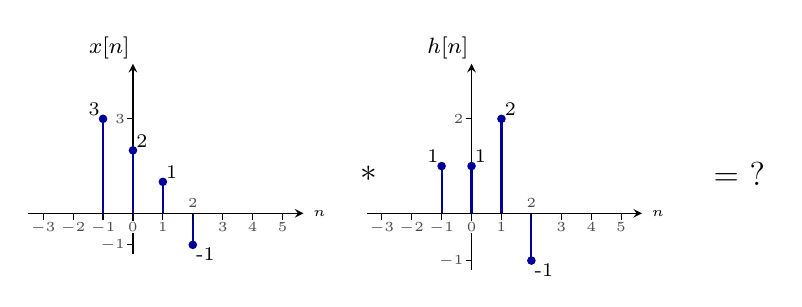
\begin{tikzpicture}[>=stealth]
  \node[font=\footnotesize] at (0.3,2.1) {$x[n]$};
  \stemat{0.6}{0}{-1}{3,2,1,-1}{0.4}
  \node[font=\large] at (3.6,0.5) {$\ast$};
  \node[font=\footnotesize] at (4.6,2.1) {$h[n]$};
  \stemat{4.9}{0}{-1}{1,1,2,-1}{0.6}
  \node[font=\large] at (8.3,0.5) {$=\ ?$};
\end{tikzpicture}
\caption{第二种问法：直接求 $x[n]\ast h[n]$。它和上一张图的第一种问法是同一道题。}
\end{figure}

\textbf{两种出题方式完全一样}。看到第二种写法，应当想到：它的意思是——如果 $\delta[n]$ 的响应是 $h[n]$，那么 $x[n]$ 的响应是什么？答案是 $y[n]=x[n]\ast h[n]$。后面会用第二种出题方式，但\textbf{第一种才是这个问题的本质}。

卷积的简便算法（教材 2.2 节）见第 \ref{sec:list}、\ref{sec:conv} 节。

\subsection{\texorpdfstring{推论：$h[n]$ 是 LTI 系统唯一的标识}{推论：h[n] 是 LTI 系统唯一的标识}}
有了 $h[n]$ 和卷积这两个名字，先看两道判断题。

\point{判断题 A。}如果两个 LTI 系统的 $h[n]$（单位脉冲响应）一样，那么这两个 LTI 系统是完全一样的。对还是错？

答案：\textbf{对}。换一种问法：如果两个 LTI 系统的 $h[n]$ 一样，那么对于任何输入，这两个系统的输出都一样——这句话是对的。（因为输出 $=x\ast h$，$h$ 一样就一样。）

两个系统对任意输入的输出都一样，它们\textbf{是同一个系统吗}？按\textbf{信号与系统这门工程学科}的理解：\textbf{如果两个系统的输入输出一样，它们就是一样的，因为没有别的办法证明它们不一样}。

\begin{remember}
\textbf{$h[n]$ 是 LTI 系统唯一的标识。}一个 LTI 系统所有的特点，都集中在 $h[n]$ 这一个序列里。
\end{remember}

\point{判断题 B（换一种问法）。}如果两个\textbf{系统}的 $h[n]$ 一样，那么这两个系统的输入输出都一样。对吗？这句话比刚才那句\textbf{少了哪个条件}？

答案：\textbf{少了「LTI」这个前提，所以不对}。$h[n]$ 是\textbf{线性时不变系统}的唯一标识，\textbf{不是所有系统}的唯一标识。原因是上面「证明」里用到的三条性质：

\begin{itemize}[nosep]
\item 用的是线性的\textbf{齐次性}（乘 $a$ 倍）；
\item 用的是\textbf{时不变性}（平移）；
\item 用的是线性的\textbf{叠加性}（相加）。
\end{itemize}
这三条都是 LTI 系统才有的。\textbf{如果不是 LTI，这些推导全是错的，这个题就做不出来。}对一个不是 LTI 的系统，$h[n]$ 不过就是「$\delta[n]$ 这个输入对应的输出」，没有什么特殊地位，只是一个普通的输入对应的输出。\textbf{只有在 LTI 系统里，$h[n]$ 才特殊。}


%==================================================================
\section{第一种算法：列表法}\label{sec:list}
算 $x[n]\ast h[n]$ 有\textbf{两种方法}，先讲第一种：\textbf{列表法}。仍用前面那道题（第 \ref{sec:draw} 节的例~\ref{ex:four}：$x=(3,2,1,-1)$ 在 $n=-1..2$，$h=(1,1,2,-1)$ 在 $n=-1..2$）。步骤：\ \textcircled{1}确定 $y[n]=x[n]\ast h[n]$ 的取值范围；\ \textcircled{2}列表；\ \textcircled{3}竖着加。

\subsection{方法：三步}
\point{第一步：确定 $y[n]$ 有值的范围。}
\begin{remember}
$y[n]$ 的\textbf{最左边} $=$ $x[n]$ 的最左边 $+$ $h[n]$ 的最左边；\\
$y[n]$ 的\textbf{最右边} $=$ $x[n]$ 的最右边 $+$ $h[n]$ 的最右边。
\end{remember}
这道题里：最左边 $(-1)+(-1)=-2$，最右边 $2+2=4$，所以 $y[n]$ \textbf{只在 $n=-2$ 到 $4$ 有值}。为什么这样，见下一小节「证明」。

\point{第二步：列表。}表格最上面一行写 $h[n]$ 的值 $1,1,2,-1$，最左边一列竖着写 $x[n]$ 的值 $3,2,1,-1$，格子里填乘积：
\begin{enumerate}[nosep]
\item 把 $h[n]$ \textbf{从左抄到右}写在最上面一行：$1,1,2,-1$。
\item 拿 $x$ 最左边的数 $3$，去乘上面 $h$ 的\textbf{每一个}：$3\times(1,1,2,-1)=(3,3,6,-3)$，写在下面一行，\textbf{和 $h$ 的位置对齐}。
\item 拿 $x$ 的第二个数 $2$，同样去乘 $h$ 的每一个，得 $(2,2,4,-2)$。\textbf{但是}：这个 $2$ 在 $x$ 里比刚才那个 $3$ \textbf{又往右挪了一位}，所以这一行的乘积也要\textbf{又往右挪一位}再写。
\item 第三个数 $1$：它比 $3$ 往右挪了两位，所以 $(1,1,2,-1)$ 要往右挪\textbf{两位}。
\item 第四个数 $-1$：往右挪三位，得 $(-1,-1,-2,1)$。
\end{enumerate}

\begin{center}
\begin{tabular}{@{}l|ccccccc@{}}
\toprule
 & \multicolumn{7}{c}{$y[n]$ 的下标 $n$}\\
 & $-2$ & $-1$ & $0$ & $1$ & $2$ & $3$ & $4$\\
\midrule
$h$（从左抄到右，对齐第一行） & $1$ & $1$ & $2$ & $-1$ & & & \\
\midrule
$3\times h$ & $3$ & $3$ & $6$ & $-3$ & & & \\
$2\times h$（右挪 1 位） & & $2$ & $2$ & $4$ & $-2$ & & \\
$1\times h$（右挪 2 位） & & & $1$ & $1$ & $2$ & $-1$ & \\
$-1\times h$（右挪 3 位） & & & & $-1$ & $-1$ & $-2$ & $1$\\
\midrule
\textbf{竖着加} & $\mathbf{3}$ & $\mathbf{5}$ & $\mathbf{9}$ & $\mathbf{1}$ & $\mathbf{-1}$ & $\mathbf{-3}$ & $\mathbf{1}$\\
\bottomrule
\end{tabular}
\end{center}

\point{第三步：竖着加。}注意：\textbf{不要把最上面那一行（$h$）也加进去}，它只是抄下来的参考行；只加下面四行。然后从最左边 $n=-2$ 开始，依次读出：$3,5,9,1,-1,-3,1$。

\subsection{证明：为什么这样做是对的}
\begin{note}
\textbf{这一张表和第 \ref{sec:draw} 节例~\ref{ex:four} 里的「拆成四个脉冲」是同一件事。}那道例题里四个输出行，每行是「$x$ 的某个值 $\times$ $h$（平移过的）」；这里的四行一模一样，只是\textbf{摆成了表格}。表格只是把那套复杂算法用简洁的形式重做了一遍，每一步都与拆脉冲的做法一一对应。
\end{note}

\point{范围规则为什么是对的。}列表法唯一需要解释的是第一步：为什么 $y$ 的最左边是 $x$ 的最左边加 $h$ 的最左边？
\begin{itemize}[nosep]
\item $x[n]=\delta[n]$ 时，输出是 $h[n]$。$h[n]$ 的最左边，相对于 $0$ 是向左挪了「$h$ 的最左边」那么多；
\item 现在 $x[n]$ 的最左边那个脉冲，本来就比 $0$ 挪了「$x$ 的最左边」那么多，它送进系统，输出（时不变性）也整体挪了这么多；
\item 所以 $y$ 的最左边，相对于 $0$，就是「$h$ 的最左边」加上「$x$ 的最左边」。最右边同理。
\end{itemize}


\subsection{例题}
\example{教材例 2-7：两个五点全 1 序列}{结果像座小山}{}
\textbf{题目}：$x[n]$ 在 $n=0..4$ 都是 $1$，$h[n]$ 也在 $n=0..4$ 都是 $1$，求 $y[n]=x[n]\ast h[n]$。

\begin{figure}[H]
\centering
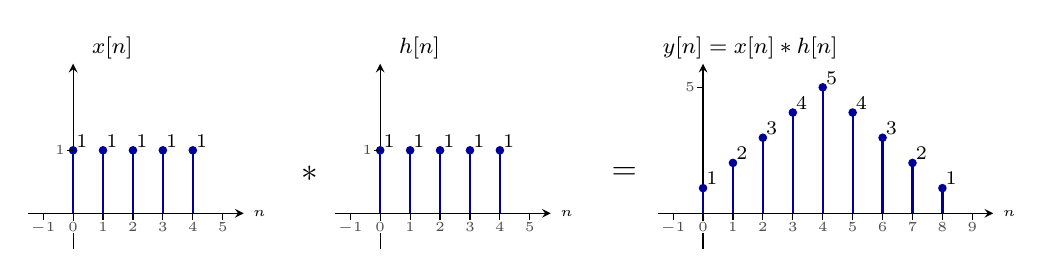
\begin{tikzpicture}[>=stealth]
  \node[font=\footnotesize] at (0.5,2.1) {$x[n]$};
  \stemr{0}{0}{0}{1,1,1,1,1}{0.8}{-1}{5}
  \node[font=\large] at (3.0,0.5) {$\ast$};
  \node[font=\footnotesize] at (4.4,2.1) {$h[n]$};
  \stemr{3.9}{0}{0}{1,1,1,1,1}{0.8}{-1}{5}
  \node[font=\large] at (7.0,0.5) {$=$};
  \node[font=\footnotesize] at (8.6,2.1) {$y[n]=x[n]\ast h[n]$};
  \stemr{8.0}{0}{0}{1,2,3,4,5,4,3,2,1}{0.32}{-1}{9}
\end{tikzpicture}
\caption{例 2-7 的题目和答案（右边是答案，纵向缩放和左边不同）。}
\end{figure}

\textbf{做法}：
\begin{enumerate}[nosep]
\item 范围：最左边 $0+0=0$，最右边 $4+4=8$，所以 $n=0..8$ 有值；
\item 列表：$x$ 的每个 $1$ 乘 $h$ 得到「5 个 $1$」，第一个 $1$ 不挪，第二个右挪 1 位，……第五个右挪 4 位；
\item 竖着加，得到 $1,2,3,4,5,4,3,2,1$，即 $n=0,1,\dots,8$ 处分别是 $1,2,3,4,5,4,3,2,1$。
\end{enumerate}
结果形状像一座小山。

\example{四点序列卷六点序列（教材第 79 页）}{结果 9 个点}{}
\label{ex:p79}\textbf{题目}（该页第一排三张图的中间一道）：$x[n]$ 在 $n=-1,0,1,2$ 处分别是 $1,2,1,1$；$h[n]$ 在 $n=0,1,2,3,4,5$ 处分别是 $1,-1,0,0,-1,1$。求 $y[n]=x[n]\ast h[n]$。

\begin{figure}[H]
\centering
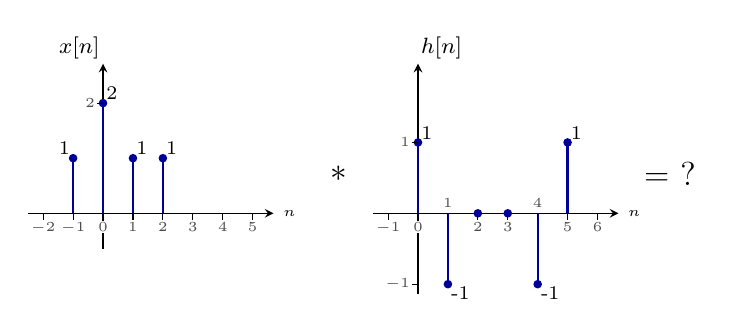
\begin{tikzpicture}[>=stealth]
  \node[font=\footnotesize] at (0.3,2.1) {$x[n]$};
  \stemr{0.6}{0}{-1}{1,2,1,1}{0.7}{-2}{5}
  \node[font=\large] at (3.6,0.5) {$\ast$};
  \node[font=\footnotesize] at (4.9,2.1) {$h[n]$};
  \stemr{4.6}{0}{0}{1,-1,0,0,-1,1}{0.9}{-1}{6}
  \node[font=\large] at (7.8,0.5) {$=\ ?$};
\end{tikzpicture}
\caption{题目：$h[n]$ 在 $n=2,3$ 处是 $0$。}
\end{figure}

答案：范围 $n=-1..7$，依次是 $1$、$1$、$-1$、$0$、$-2$、$-1$、$1$、$0$、$1$。

\begin{figure}[H]
\centering
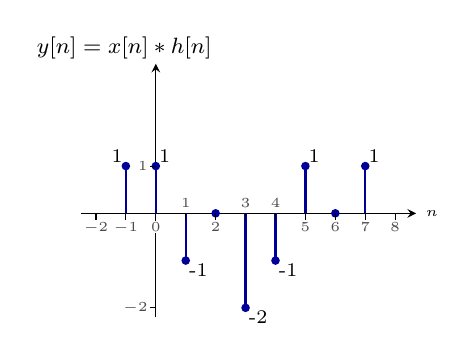
\begin{tikzpicture}[>=stealth]
  \node[font=\footnotesize] at (0.6,2.1) {$y[n]=x[n]\ast h[n]$};
  \stemr{1.0}{0}{-1}{1,1,-1,0,-2,-1,1,0,1}{0.6}{-2}{8}
\end{tikzpicture}
\caption{答案：$y[n]$ 在 $n=-1..7$ 共 9 个点。}
\end{figure}

\point{换一种出题方式：把序列写成脉冲的和。}同一道题也可能写成脉冲和的形式：
\begin{align*}
x[n]&=\delta[n+1]+2\delta[n]+\delta[n-1]+\delta[n-2],\\
h[n]&=\delta[n]-\delta[n-1]-\delta[n-4]+\delta[n-5],\\
y[n]&=x[n]\ast h[n].
\end{align*}
\textbf{这和上面那道题是同一道题。}$\delta[n-m]$ 就是「在 $n=m$ 处放一个 $1$」，前面的系数就是那一点的值。只要理解 $\delta$ 的性质和左右移的写法，它就是同一道题。

\example{无限长的序列：教材例 2-6}{找规律}{}

\textbf{题目}：$x[n]=a^n u[n]$，$h[n]=u[n]$，求 $y[n]=x[n]\ast h[n]$。其中 $u[n]$ 是\textbf{单位阶跃序列}(unit step sequence)：$n\ge0$ 时为 $1$，$n<0$ 时为 $0$。要有解，需要 $|a|<1$。

$x$ 和 $h$ 都是无限长时，列表法\textbf{仍然可以用}：把前几项算出来，\textbf{总结规律}，再写出统一的表达式。

\paragraph{步骤。}
\begin{enumerate}[nosep]
\item \textbf{先把 $x$ 和 $h$ 大致画出来}：$x[n]$ 在 $n<0$ 时是 $0$，$n\ge0$ 时是 $1,a,a^2,a^3,\dots$（$a^n u[n]$ 里 $u[n]$ 把负半边「切掉」）；$h[n]=u[n]$ 是 $n\ge0$ 时一直是 $1$ 的序列。
\item \textbf{范围}：最左边 $0+0=0$，最右边 $+\infty$，所以 $y[n]$ 在 $n\ge0$ 有值。
\item \textbf{列表}：这张表向右、向下都无限延伸。$x$ 的第一个数 $1$ 乘 $h$：一行全是 $1$；第二个数 $a$，右挪一位，一行全是 $a$；第三个数 $a^2$，再右挪一位，一行全是 $a^2$；……
\item \textbf{先加前几项找规律}：竖着加，
  \begin{center}
  \begin{tabular}{@{}c|l@{}}
  \toprule
  $n$ & 竖着加的结果\\
  \midrule
  $0$ & $1$\\
  $1$ & $1+a$\\
  $2$ & $1+a+a^2$\\
  $3$ & $1+a+a^2+a^3$\\
  \bottomrule
  \end{tabular}
  \end{center}
\item \textbf{写成统一的式子}：$n\ge0$ 时 $y[n]=1+a+a^2+\cdots+a^n$。但 $n<0$ 时应该是 $0$，所以\textbf{前面要乘一个 $u[n]$}（乘上后 $n<0$ 时全为 $0$）：
  \[y[n]=\bigl(1+a+a^2+\cdots+a^n\bigr)u[n].\]
\item \textbf{用等比数列求和公式化简}（分子分母同乘 $1-a$，$(1-a)(1+a+\cdots+a^n)=1-a^{n+1}$）：
  \[y[n]=\frac{1-a^{n+1}}{1-a}\,u[n].\]
\end{enumerate}
写成上一步（未化简）的形式也正确。学完第 4 章和第 7 章之后，\textbf{用傅里叶变换和 $z$ 变换会非常快}；用找规律的办法也不难。

\point{两个思考题：卷积的长度与计算量。}

\example{卷积后序列有多长？}{\texorpdfstring{$N_1+N_2-1$}{N1+N2-1}}{}
\textbf{题目}：若 $x[n]$ 的长度是 $N_1$（即非零值连续排列、共 $N_1$ 个），$h[n]$ 的长度是 $N_2$，问 $y[n]=x[n]\ast h[n]$ 的长度是多少？

\textbf{解}：举个例子即可。设 $x[n]$ 在 $0$ 到 $N_1-1$ 有值（长度正好是 $N_1$），$h[n]$ 在 $0$ 到 $N_2-1$ 有值，用「最左加最左，最右加最右」，$y[n]$ 在 $0$ 到 $(N_1-1)+(N_2-1)=N_1+N_2-2$ 有值，所以长度是
\begin{remember}
长度 $N_1$ 的序列和长度 $N_2$ 的序列卷积，结果的长度是 \textbf{$N_1+N_2-1$}。
\end{remember}
起点不一定是 $0$，换别的起点长度也一样。检查：第 \ref{sec:draw} 节例~\ref{ex:four} 那道题 $4+4-1=7$，正好是 $n=-2..4$ 共 7 个点；例 2-7 是 $5+5-1=9$ 个点。

\example{列表法要算多少次加法、多少次乘法？}{\texorpdfstring{$O(N^2)$}{O(N的平方)}}{}
\textbf{题目}：$x[n]$ 长度为 $N$，$h[n]$ 长度也为 $N$，用列表法算 $y[n]=x[n]\ast h[n]$，需要多少次\textbf{加法}、多少次\textbf{乘法}？

用 $N=4$ 的那张表来数：
\begin{itemize}[nosep]
\item \textbf{乘法}：表里每个格子都是一次乘法，有 $N$ 行、每行 $N$ 个，共 \textbf{$N^2$ 次}乘法；
\item \textbf{加法}：竖着加，每一列要加几次，看那一列有几个数：从左到右，各列需要的加法次数是 $0,1,2,3,2,1,0$（头尾两列只有一个数，不用加）。即 $1+2+3+2+1$，对 $N$ 来说就是
  \[1+2+\cdots+(N-1)+(N-2)+\cdots+1=(N-1)^2.\]
  当 $N=4$ 时是 $9$。
\end{itemize}
所以用列表法做卷积，\textbf{计算复杂度是 $O(N^2)$}（加法和乘法的次数大致正比于 $N^2$）。

\paragraph{能不能把加法和乘法的次数减少？}能。Cooley 和 Tukey（1965 年）提出的\textbf{快速傅里叶变换}(fast Fourier transform，FFT)，把卷积的计算复杂度从 $O(N^2)$ 降到 $O(N\log N)$，第四章会学。这是信号处理领域非常重要的发现，初看却很反直觉：加法和乘法从哪里省下来，并不明显。

\paragraph{差距有多大。}实际用卷积时，序列常有几万、几十万甚至几百万长。取 $N=10^5$：
\begin{center}
\begin{tabular}{@{}lll@{}}
\toprule
 & 算法 & 次数（数量级）\\
\midrule
列表法 & $N^2$ & $(10^5)^2=10^{10}$\\
FFT & $N\log N$ & $10^5\log10^5=5\times10^5$\\
\bottomrule
\end{tabular}
\end{center}
$N$ 越大，差距越大。（这里 $\log$ 取以 $10$ 为底，$\log10^5=5$；$O(N\log N)$ 里底数不影响数量级。）


%==================================================================
\section{第二种算法：卷积公式法}\label{sec:conv}
\subsection{概念}
用卷积公式还有另一种算法，叫\textbf{卷积公式法}。分\textbf{四步}（教材分五步，这里合为四步）：
\begin{center}
\textbf{翻转 \;\; 平移 \;\; 相乘 \;\; 求和}
\end{center}

\point{用卷积公式法要注意的两点。}
\begin{remember}
\begin{enumerate}[nosep]
\item 这里\textbf{翻转 $h[n]$}。也可以翻转 $x[n]$，因为\textbf{卷积具有交换性}（后面证明）。
\item \textbf{翻转谁，就平移谁，不要反过来。}翻转 $h$ 就平移 $h$；翻转 $x$ 就平移 $x$。若翻转 $h$ 却去平移 $x$，就错了。
\end{enumerate}
\end{remember}

\subsection{证明：四步从哪里来}
把公式里的 $h[n-k]$ 稍微变一下形：$n-k=-(k-n)$，所以
\[
x[n]\ast h[n]=\sum_{k=-\infty}^{+\infty}x[k]\;h\bigl[-(k-n)\bigr].
\]
四步与公式的对应：

\begin{center}
\begin{tabular}{@{}p{1.4cm}p{4.0cm}p{9.2cm}@{}}
\toprule
步骤 & 在公式里在哪里 & 意思\\
\midrule
\textbf{翻转} & $h[\,\textbf{-}(k-n)]$ 里的\textbf{负号} & 把 $h[k]$ 左右翻过来，变成 $h[-k]$（从右抄到左）\\
\textbf{平移} & $h[-(k-\textbf{n})]$ 里的 $n$ & \textbf{右移 $n$ 个单位}（减号表示右移；$n$ 为负数时，右移 $n$ 个单位等于左移 $|n|$ 个单位）\\
\textbf{相乘} & $x[k]\cdot h[\cdots]$ 两个相乘 & 翻转并平移后的 $h$，和 $x[k]$ 逐点相乘\\
\textbf{求和} & $\displaystyle\sum_{k}$ & 把所有乘积加起来，得到 $y[n]$ 在这一个 $n$ 的值\\
\bottomrule
\end{tabular}
\end{center}
这里的「翻转」和「平移」，就是第一章「信号的自变量变换」里讲的那一套。

\subsection{例题}
\example{用公式法重做四点输入的题}{与列表法一致}{}
\textbf{题目}（即第 \ref{sec:draw} 节例~\ref{ex:four}）：$x[n]=(3,2,1,-1)$ 在 $n=-1..2$，$h[n]=(1,1,2,-1)$ 在 $n=-1..2$，求 $x[n]\ast h[n]$。

\paragraph{第一步，和列表法完全一样：确定范围。}$y$ 的最左边 $(-1)+(-1)=-2$，最右边 $2+2=4$，所以 $n=-2..4$ 有值。关键是后面这些值怎么算。

\paragraph{第二步：把 $h$ 翻转。}$h[n]$ 从左抄到右是 $1,1,2,-1$；翻转的意思是\textbf{把它从右抄到左}，也就是 $h[-n]$：从左到右写是 $-1,2,1,1$。

\paragraph{第三步：不断平移、相乘、求和。}把 $x$ 从左抄到右写好（$3,2,1,-1$），再把翻转过的 $h$（$-1,2,1,1$）\textbf{一格一格往右挪}，每挪一格，就把\textbf{重合在一起的数两两相乘再相加}，得到 $y$ 在这一个位置的值：

\begin{center}
\begin{tabular}{@{}c|p{4.3cm}|p{5.2cm}|c@{}}
\toprule
$n$ & 重合的数（上面 $x$，下面翻转后的 $h$） & 乘积 & 相加\\
\midrule
$-2$ & $3$ 和 $1$ & $3\times1$ & $3$\\
$-1$ & $3,2$ 和 $1,1$ & $3\times1+2\times1$ & $5$\\
$0$ & $3,2,1$ 和 $2,1,1$ & $3\times2+2\times1+1\times1$ & $9$\\
$1$ & $3,2,1,-1$ 和 $-1,2,1,1$ & $3\times(-1)+2\times2+1\times1+(-1)\times1$ & $1$\\
$2$ & $2,1,-1$ 和 $-1,2,1$ & $2\times(-1)+1\times2+(-1)\times1$ & $-1$\\
$3$ & $1,-1$ 和 $-1,2$ & $1\times(-1)+(-1)\times2$ & $-3$\\
$4$ & $-1$ 和 $-1$ & $(-1)\times(-1)$ & $1$\\
\bottomrule
\end{tabular}
\end{center}
（$n=-2$ 时：翻转的 $h$ 最右边的 $1$ 和 $x$ 最左边的 $3$ 对上；每挪一格，多一个数重合，直到 4 个全重合，再逐渐退出。）

结果是 $3,5,9,1,-1,-3,1$，\textbf{和列表法、和第 \ref{sec:draw} 节例~\ref{ex:four} 的蛮力法完全一样}，正是公式所描述的内容。

\point{用公式法重做例 2-7、例 2-6。}

\example{教材例 2-7（公式法）}{与列表法一致}{}
这次题目写成
\[x[n]=u[n]-u[n-5],\qquad h[n]=u[n]-u[n-5],\qquad\text{求 }x[n]\ast h[n].\]
$u[n]$ 从 $0$ 起一直是 $1$，$u[n-5]$ 从 $5$ 起一直是 $1$，相减只剩 $n=0..4$ 的 5 个 $1$——就是例 2-7。
\begin{enumerate}[nosep]
\item 范围 $n=0..8$；
\item $h$ 翻转后还是 5 个 $1$（所以 $h[-n]$ 也是 5 个 1）；
\item 往右挪：$n=0$ 时只有一个 $1$ 对上，得 $1$；右挪 1 格，两对，得 $2$；……右挪 4 格，五对全重合，得 $5$；再往右，重合数逐渐减少，$4,3,2,1$。
\end{enumerate}
得到的结果和列表法的 $1,2,3,4,5,4,3,2,1$ 一致。

\example{教材例 2-6（公式法）}{与列表法一致}{}
$x[n]=a^nu[n]$，$h[n]=u[n]$。范围 $n\ge0$；把 $h$ 翻转，往右挪，$n=0$ 时只有 $x[0]=1$ 一项，$n=1$ 时 $1+a$，$n=2$ 时 $1+a+a^2$，……得到的规律
\[
y[n]=(1+a+\cdots+a^n)u[n]=\frac{1-a^{n+1}}{1-a}u[n],
\]
和列表法一样。核心就是翻转、平移、相乘、求和，即卷积公式本身。

%==================================================================
\section{列表法和卷积公式法，哪个更好？}
两种方法都能算出正确结果，用哪一种都可以。两者各有优劣：
\begin{itemize}[nosep]
\item \textbf{列表法更快}：不需要「翻转以后再写」。
\item \textbf{但列表法有个最大的问题}：\textbf{错了一个数，基本上整张表都错}。
\item \textbf{卷积公式法是一个一个算}：比如 $y[0]$ 算错，$y[1]$、$y[2]$ 仍可能算对。
\end{itemize}
一个有意思的观察：在人看来，列表法和卷积公式法各有优劣；\textbf{在计算机眼里，是同一个方法}。两种方法\textbf{加法和乘法的次数完全一样}，只是\textbf{顺序}不同，所以时间复杂度也一样。

\begin{note}
\textbf{为什么是同一个方法}：两种方法都要把每个 $x[k]$ 和每个 $h[m]$ 配一次对、乘一次（共 $N^2$ 次乘法），再把落在同一个 $n=k+m$ 上的乘积加起来。列表法是「一行一行乘，最后竖着加」，卷积公式法是「一个 $n$ 一个 $n$ 地乘再加」，只是\textbf{先算哪个、后算哪个}不一样。
\end{note}

\end{document}
